\documentclass[10pt]{article}
\usepackage{pictex,amsmath,amsfonts,amssymb,amsthm,verbatim}
\usepackage{fullpage}
\usepackage{algorithm,algorithmic}
\usepackage{gensymb}
\usepackage{mathrsfs}

\setlength{\voffset}{-0.25in}
\setlength{\headsep}{+0.5in}
\setlength{\parskip}{1em}
\setlength{\parindent}{0em}

\def\vu{\mathbf{u}}
\def\vv{\mathbf{v}}
\def\vb{\mathbf{b}}
\def\vw{\mathbf{w}}
\def\vs{\mathbf{s}}

%Font:
\usepackage{lmodern}
\renewcommand*\familydefault{\sfdefault} %% Only if the base font of the document is to be sans serif
\usepackage[T1]{fontenc}

%Graphics packages:
\usepackage{graphicx, graphics}
\usepackage{tabularx, caption}
\usepackage{multirow, multicol}
\usepackage{setspace, tikz}
\usepackage{xcolor}
\usepackage{titlesec}
\usepackage{mdframed}
\usepackage{fancyhdr}
\usepackage{lastpage}
\usepackage[utf8]{inputenc}

%Box:
\newmdenv[linecolor=blue,
          skipabove=\topsep,
          skipbelow=\topsep,
          leftmargin=5pt,
          rightmargin=-5pt,
          innerleftmargin=5pt,
          innerrightmargin=5pt]{mybox}

%Minted (for code):
\usepackage{minted}
\newminted{C}{frame = lines, framerule = 2pt}
          
%Macro:
\newcommand{\quotes}[1]{``#1''}
\newcommand{\tf}{\textbf}
\newcommand{\ti}{\textit}
\newcommand{\ttt}{\texttt}
\newcommand{\ud}{\underline}
\newcommand{\rarrow}{\rightarrow}
\newcommand{\larrow}{\leftarrow}
\newcommand{\lrarrow}{\leftrightarrow}

\pagestyle{fancy}
\fancyhead{}
\fancyfoot{} %clear all footer fields
\fancyfoot[L]{\scriptsize \ttfamily CC01 - Operating System}
\fancyfoot[R]{\scriptsize \ttfamily Page {\thepage}/ \pageref{LastPage}}
\renewcommand{\headrulewidth}{0pt}
\renewcommand{\footrulewidth}{0.3pt}


\begin{document}

\begin{center}
\Huge Operating System 
\bigbreak
\large Pham Minh Tuan - 1752595
\end{center}

%Table of contents:
\renewcommand*\contentsname{Contents:}
\tableofcontents

%Newpage
\newpage

\section{Overview}

\quotes{What is Operating System ?}
\begin{itemize}
	\item An operating system acts an intermediary(trung gian) between the user of a computer and the computer hardware.
	\item Operating system provide an environment in which a user can execute programs in a \textit{convenient} and \textit{efficient} manner.
	\item An Operating System is software that manages the computer hardware, the hardware must provide appropriate mechanisms to ensure the correct operation and prevent user from interfering with the proper operation of the system.
\end{itemize}

\subsection{What Operating System can do ?}
\begin{enumerate}
	\item A computer system can be divided into 4 components: the \textbf{hardware}, the \textbf{operating system}, the \textbf{application programs}, and the \textbf{users}.
	\begin{itemize}
		\item The Hardware includes the \textbf{central unit processing} (CPU), the \textbf{memory}, and the \textbf{input-output} (IO) \textbf{devices}
		\item Hardware provides the basic computing resources for the system.
		\item The Application programs define the ways in which these resources are used to solve user's computing problem.
		\item The operating system controls the hardware and coordinates it use among the various application programs for various users.
		\item In system's view, the operating system is the program most intimately involved with the hardware. an operating system can be viewed as \textbf{resource allocator}.
		\item An operating system is a control program that manages the execution of user programs to prevent errors and improper use of the computer.
		\item An operating system is a program running at all times on the computer - usually called the \textbf{kernel}
	\end{itemize}

	\item \textbf{Computer-System Operation} 
	\begin{itemize}
		\item For a computer to start running, it needs to have an initial program to run or \textbf{bootstrap program}.
		\item Bootstrap program is stored in \textbf{ROM} (read-only memory) or \textbf{EEPROM} (electrically erasable programmable read-only memory) or \textbf{firmware}.
		\item Bootstrap program initializes all aspects of the system, it knows how to load the operating system and start executing that system.
		\item The operating system then starts executing the first process and waits for the occurrence events.
		\item The occurrence of an event is usually signaled by an \textbf{interrupt} from either software or hardware.

		\begin{itemize}
			\item Hardware may trigger an interrupt at any time by sending a signal to the CPU.
			\item Software may trigger a special operation called a \textbf{system call} or \textbf{monitor call}.
		\end{itemize}

	\end{itemize}

	\item \textbf{Interrupt: }
	\begin{itemize}
		\item When the CPU is interrupted, it stops what it is doing and immediately transfers execution to a fixed location.
		\item The fixed location usually contains the starting address where service routine for the interrupt is located.
		\item The interrupt must transfer control to the appropriate interrupt service routine.
		\item The \textbf{interrupt vector} provide the address of the interrupt service routine for the interrupting device.
		\item The interrupt architecture must also save the address of the interrupted instruction.
		\item Incoming interrupts are disabled while another interrupt is being processed to prevent a \textbf{lost interrupt}
		\item A \textbf{trap} is a software-generated interrupt caused either by an error or a user request.
		\item An operating system is \textbf{interrupt driven}. 
	\end{itemize}

	\item \textbf{Storage Structure}
	\begin{itemize}
		\item General-purpose computers run most of their program from rewritable memory, called main memory (or random-access memory (RAM)).
		\item Main memory is commonly implemented in a semiconductor technology called \textbf{dynamic random-access memory} (DRAM).
		\item Main memory is usually too small to store all needed programs and data permanently.
		\item Main memory is a \textit{volatile} storage device that loses its contents when power is turned off or otherwise lost.
		$\rightarrow$ \textbf{secondary storage} for larges quantities of data permanently.
		\item \textbf{magnetic disk}: provide storage for both program and data.
		\item Most programs (system and application) are storage on a disk until they are loaded into memory.
		\item Differences between among the various storage systems lie on speed, cost, size and volatility.

		\bigbreak
		%\includegraphics[scale = 0.3]{hinh.png}
		\bigbreak

		\item In the absence of power and general backup systems, some data must be written to \textbf{nonvolatile storage}.
		\item Some nonvolatile disks are electronic disk, NVRAM (DRAM with battery backup power).
	\end{itemize}

\end{enumerate}

\pagebreak
\section{Chapter 3: Process}

\subsection{Process Concept}
\begin{enumerate}
	\item \textbf{The Process}
	\begin{itemize}
		\item The process:
		\begin{itemize}
			\item A process is a program in execution.
			\item The status of the current activity of a process is represented by the value of the \textbf{program counter} and the contents of the processor's register. 
			\item The memory layout of a process is typically divided into multiple sections
			\begin{itemize}
				\item \textbf{Text section:} - the executable code 
				\item \textbf{Data section:} - global variables
				\item \textbf{Heap section:} - memory that is dynamically allocated duirng program run time.
				\item \textbf{Stack section:} - temporary data storage when invoking functions (parameters, return val, ... etc).
				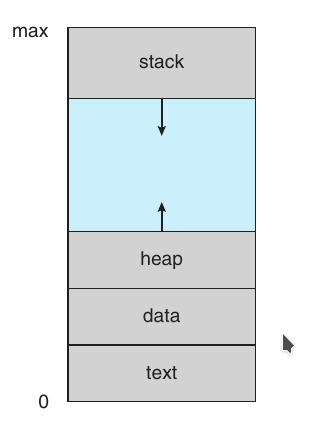
\includegraphics[width=5cm]{memory_layout.png}
				\bigbreak
			\end{itemize}

			\item The size of text and data section is \textbf{fixed}, while the stack and heap section can shrink and grow \textbf{dynamically} during program execution.
			\item the stack and heap sections grow \textbf{toward} one another, the operating system must ensure they do not \textbf{overlap} one another.
			\item A program itself is not a process, which is called \textbf{passive entity} while process is called \textbf{active} entity with a program counter specifying the next instruction to execute and a set of associated resources.
			\item A program become a process when when an executable file is loaded into a memory.
			\item Two processes may be associated with the same program, they are nevertheless considered two separate execution sequences.
			\item A process can itself be an execution environment for another code. For instance, the JVM   
		\end{itemize}
	\end{itemize}

	\item \textbf{Process State}
	\begin{itemize}
		\item The state of the process is defined in part of the current activity of that process.
		\begin{itemize}
			\item \textbf{New}: The process is being created.
			\item \textbf{Running}: Instructions are being executed.
			\item \textbf{Waiting}: The process is waiting for some events to occur (such as I/O completion or reception of a signal).
			\item \textbf{Ready}: The process is waiting to be assigned to a processor.
			\item \textbf{Terminated}: The process has finished execution.
		\end{itemize}

		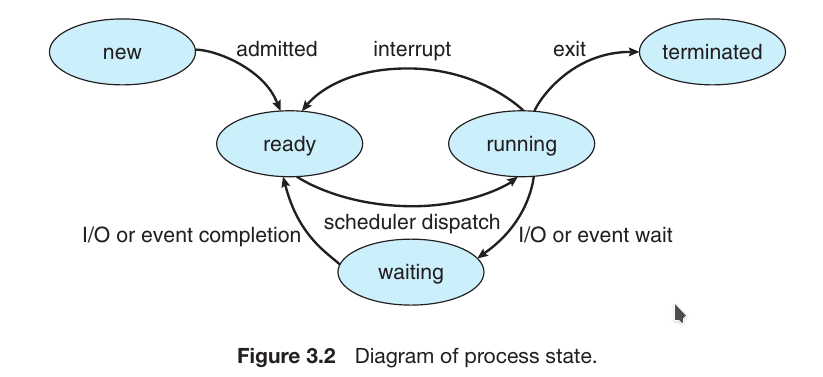
\includegraphics[scale=0.6]{Process_state.png}
		\\
		\bigbreak

		\item Only \textbf{one} process can be \textit{running} on any processor core at any instant. Many process may be \textit{ready} and \textit{waiting}. 
	\end{itemize}

	\item \textbf{Process Control Block}
	\begin{itemize}
		\item Each process is represented in the operating system by a \textbf{process control block (PCB)} or \textbf{task control block}.
		\begin{itemize}
			\item Process state
			\item Program counter
			\item CPU register
			\item CPU-scheduling information
			\item Memory-management information
			\item Accounting information
			\item I/O status information
		\end{itemize}
	\end{itemize}

	\item \textbf{Threads}
	\begin{itemize}
		\item A process is a program that performs a single \textbf{thread} of execution.
	\end{itemize}
\end{enumerate}

\subsection{Process Scheduling}

\begin{itemize}
	\item The objective of multiprogramming is to have some process running at all the times so as to maximize CPU utilization.
	\item The objective for time sharing is to switch a CPU core among processes so frequently that users can interact with each program while it is running.
	\item To meet those objective, \textbf{process scheduler} is used to select an available process for program execution on a core.
	\item The number of processes currently in memory is known as the \textbf{degree of multiprogramming}.
	\item Most processes can be described as either I/O bound or CPU bound.
	\begin{itemize}
		\item An \textbf{I/O bound process} is one that spends more of its time doing I/O than it spends doing computations.
		\item A \textbf{CPU-bound process} generates I/O requests infrequently, using more of its time doing computations. 
	\end{itemize}
\end{itemize}

\begin{enumerate}
	\item \textbf{Scheduling Queues}
	\begin{itemize}
		\item As a processes enter the system, they are put into the \textbf{ready queue}, where they are ready and waiting to execute on a CPU's core. This queue is a linked-list.
		\item When a process is allocated a CPU core, it executes for a while and eventually terminates, is interrupted, or waits for the occurrence of a particular event - I/O request. Therefore, the process has to wait for the completion of I/O - which is placed in a \textbf{wait queue}. 
	\end{itemize}

	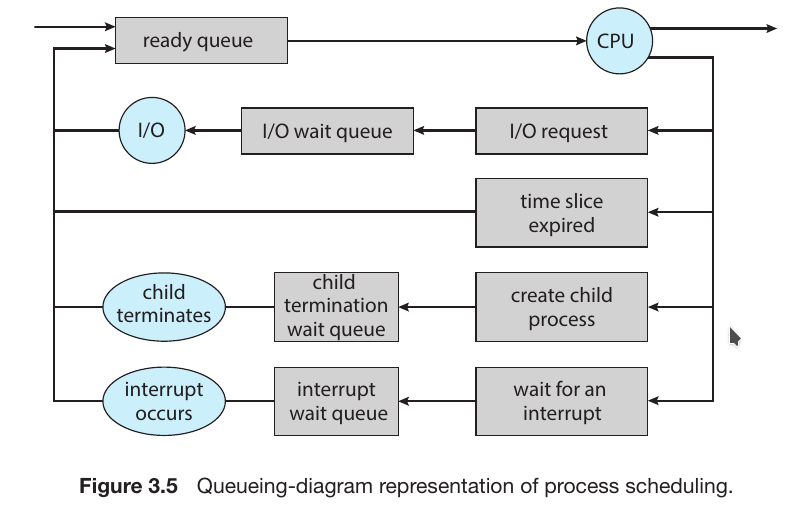
\includegraphics[scale=0.6]{Queueing-diagram.png}
	\\
	\bigbreak

	\item \textbf{CPU Scheduling}
	\begin{itemize}
		\item The role of \textbf{CPU scheduler} is to select from among the processes that are in the ready queue and allocate a CPU core to one of them.
		\item The scheduler must select a new process for the CPU frequently.
	\end{itemize}
\end{enumerate}

\subsection{Schedulers}

\begin{itemize}
	\item \tf{Long-term scheduler} (or \tf{job scheduler}): 
	\begin{itemize}
		\item Selects which processes should be brought into the ready queue.
		\item It is invoked very \tf{frequently} (milliseconds) $\rarrow$ fast.
	\end{itemize}
	\item \tf{Short-term scheduler} (or \tf{CPU scheduler}):
	\begin{itemize}
		\item Selects which process should be executed next and allocates CPU.
		\item It is invoked very \tf{infrequently} (seconds, minutes) $\rarrow$ slow.
	\end{itemize}

	\item The long-term scheduler controls the \tf{degree of multiprogramming}.
	\item Processes can be described as:
	\begin{itemize}
		\item \tf{I/O-bound process}: spends more time doing I/O than computations, many short CPU bursts.
		\item \tf{CPU-bound process}: spends more time doing computations than I/O; few very long CPU bursts.
	\end{itemize}
\end{itemize}

\subsection{Context Switch}

\begin{itemize}
	\item When a CPU switches to another process, the system must save the state of the old process and load the saved state for the new process via \tf{context switch}.
	\item \tf{Context} of a process represented in the PCB.
	
	\bigbreak
	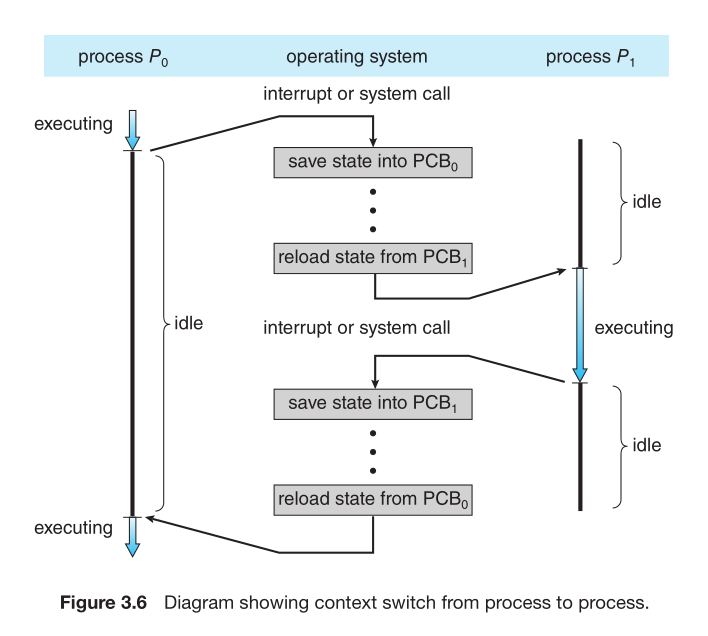
\includegraphics[scale = 0.7]{ContextSwitch.png}
	\bigbreak
\end{itemize}

\subsection{Process Creation}

\begin{itemize}
	\item \tf{Parent} process create \tf{children} processes, which in turn create other processes $\rarrow$ formming a tree of process :).
	\item Generally process is identified via \tf{a process identifier} (PID).
	\item Resource sharing:
	\begin{itemize}
		\item Parent and children share all resources.
		\item Children share subset of parent's resources.	
	\end{itemize}

	\item Execution:
	\begin{itemize}
		\item Parent and children execute concurrently.
		\item Parent waits until child terminates.
	\end{itemize}

	\item Address space of child process duplicate of parent; child has a program load into it.
	\item \tf{fork()} system call creates new process which is an exact duplicate of the calling process at the time of its creation.
	
	\bigbreak
	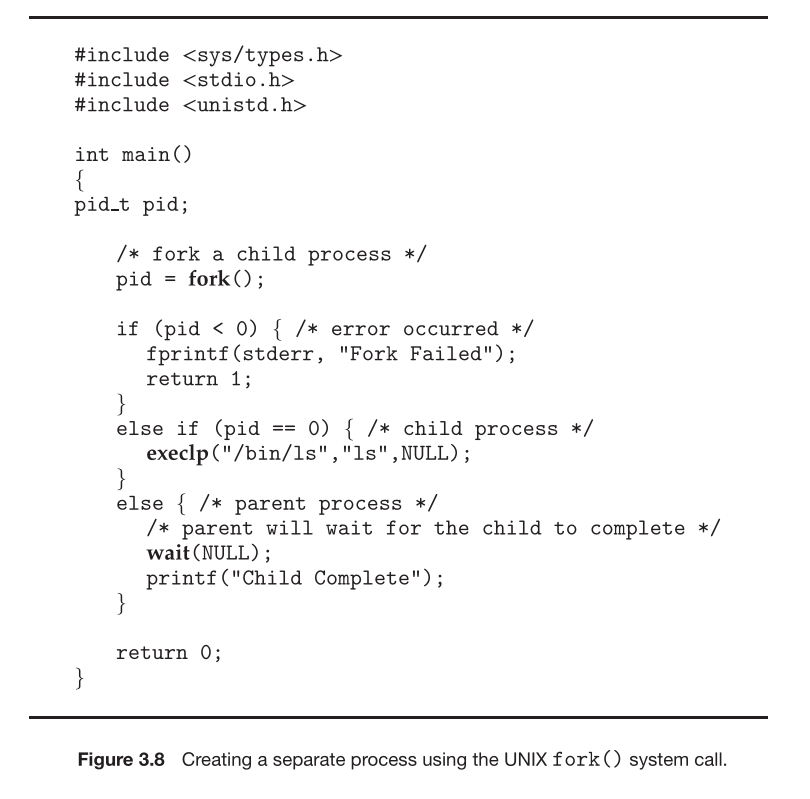
\includegraphics[scale = 0.7]{fork.png}
	\bigbreak

	\item \tf{exec()} system call used after a \tf{fork()} system call to replace the process's memory space with the new program.
	
	\bigbreak
	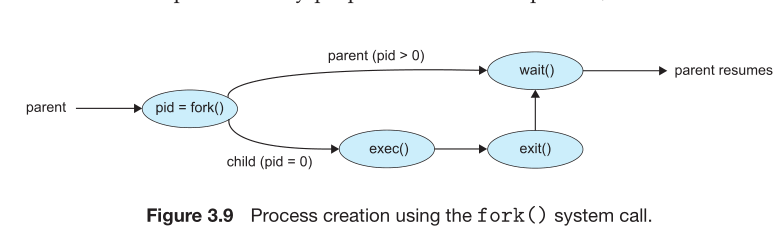
\includegraphics[scale = 0.7]{fork_exec.png}
	\bigbreak
\end{itemize}

\subsection{Process Termination}

\begin{itemize}
	\item A process terminates when it finishes executing its final statement and asks the operating system to delete it by using the \tf{exit()} system call. 
	\item At that point, the process may return a status value (typically an integer) to its waiting parent process (via the wait() system call).
	\item All the resources of the process including physical and virtual memory, open files, and I/O buffers—are de-allocated and reclaimed by the operating system.
	\item Parent may terminate execution of children processes if: 
	\begin{itemize}
		\item Child has exceed allocated resources.
		\item Task assigned to child is no longer required.
		\item if parent is exiting $\rarrow all children terminated$ (\tf{cascading termination}).
	\end{itemize}
\end{itemize}

\subsection{Interprocess Communication}

\begin{itemize}
	\item Processes within a system may be \tf{independent} or \tf{cooperating}.
	\item Cooperating process can affect or be affected by other processes, including sharing data.
	\item Reasons for cooperating processes: 
	\begin{itemize}
		\item Information sharing.
		\item Computation speedup.
		\item Modularity.
		\item Convenience.
	\end{itemize}

	\item \tf{Independent} process \tf{cannot} affect or be affected by the execution of another process.
	\item \tf{Cooperating} process \tf{can} affect or be affected by the another process.
\end{itemize}

\begin{center}
	End
\end{center}

\newpage
\section{Threads}

\begin{itemize}
	\item A thread is a basic unit of CPU utilization; it comprises a thread ID, a program counter (PC), a register set, and a stack.
	\item It shares with other threads belonging to the same process:
	\begin{itemize}
		\item code section.
		\item data section.
		\item other operating system resources, such as open files and signals.
		\item A traditional process has a single thread of control; If a process has multiple threads of control, it can perform more than one task at a time.
	\end{itemize}
\end{itemize}

\subsection{Motivation}

\begin{itemize}
	\item Threads run within application.
	\item Multiple tasks with the application can be implemented by separate threads: 
	\begin{itemize}
		\item Update display.
		\item Fetch data.
		\item Spell checking
		\item Answer a network request.
	\end{itemize}

	\item Process creation is \tf{heavy-weight} while thread creation is \tf{light-weight}
	\item Kernels are generally multithreaded.
\end{itemize}

\subsection{Multicore Programming}

\begin{itemize}
	\item Multicore systems put pressure on programmers, challenges:
	\begin{itemize}
		\item Dividing activities.
		\item Balance.
		\item Data splitting.
		\item Data dependency.
		\item Testing and debugging.
	\end{itemize}
\end{itemize}

\subsection{User Threads}

\begin{itemize}
	\item Thread management is done by user-level threads library.
	\item Three primary thread libraries:
	\begin{itemize}
		\item POSIX \tf{Pthreads}.
		\item Win32 threads.
		\item Java threads.
	\end{itemize}
\end{itemize}

\subsection{Kernel Threads}

\begin{itemize}
	\item Supported by kernel.
	\item Window, Solaris, Linux, MAC OS, etc. 
\end{itemize}

\subsection{Multithreading Models}

\begin{itemize}
	\item Many-to-One (Solaris, GNU)
	\item One-to-One (Window, Linux)
	\item Many-to-Many. (Solaris 9, Window NT/2000)
\end{itemize}

\bigbreak
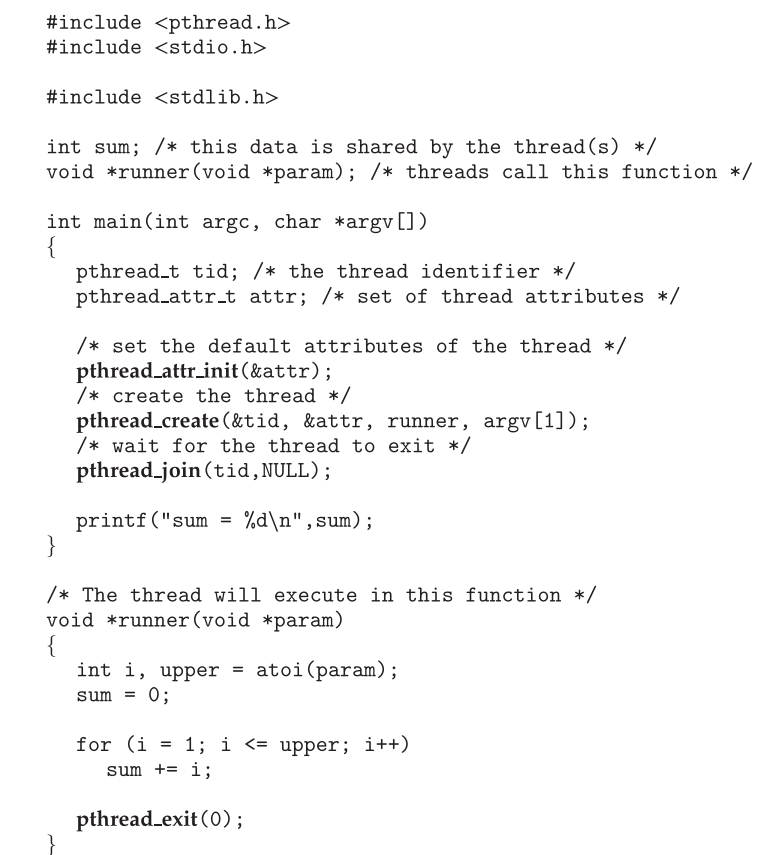
\includegraphics[scale = 0.7]{phtread.png}
\bigbreak

\subsection{Linux Threads}

\begin{itemize}
	\item Thread creation is done through \tf{clone()} system call.
	\item \tf{clone()} allows a child task to share the address space of the parent task (process).
	\item \tf{struct \ttt{task\_struct}} points to process data structures (shared or unique)
\end{itemize}

\subsection{Thread Cancellation}

\begin{itemize}
	\item \tf{Asynchronous cancellation} terminates the target thread immediately.
	\item \tf{Feferred cacellation} allows the target thread to periodically check if it should be cancelled.
\end{itemize}

\subsection{Thread Pools}

\begin{itemize}
	\item Create a number of threads in a pool where they await for works.
	\item Advantages:
	\begin{itemize}
		\item Usually slightly faster to service a request with an existing thread than create a new thread.
		\item Allows the number of threads in the application(s) to be bound to the size of the pool. 
	\end{itemize}
\end{itemize}

\subsection{Thread vs Process}

\bigbreak
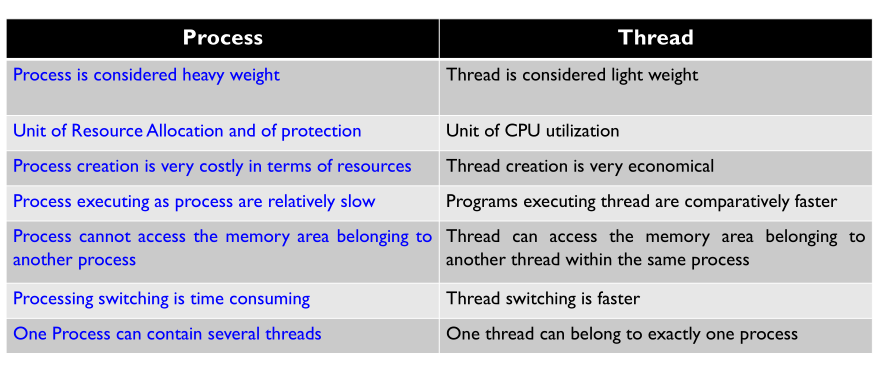
\includegraphics[scale = 0.7]{ThreadvsProcess.png}
\bigbreak

\newpage 
\section{Process Synchronization}

\subsection{Background}

\begin{itemize}
	\item \tf{Concurrent access} to shared data may result in \tf{data inconsistency}
	\item Maintaining the data consistency requires mechanism to ensure the \tf{orderly execution} of cooperating process.
\end{itemize}

\subsection{Critical Section}

\begin{minted}{cpp}
	do{
		entry section
		critical section
		exit section

		remainder section
	} while(1);
\end{minted}

\begin{itemize}
	\item Mutual Exclusion: If process Pi is executing in it critical section, then \tf{no other processes} can be executing in their critical sections.
	\item Progress: If no process is in its critical section or some processes that wish to enter their critical section,then \tf{one} process will enter the critical section.
	\item Bounded Waiting: A bound must exist on the number of times that other processes are allowed to enter their critical sections after a process has made a request to enter its
	critical section.
\end{itemize}

\subsection{Peterson's Solution}

\begin{itemize}
	\item two processes solution.
	\item Two processes share two variables:
	\begin{minted}{C}
		int turn;
		bool falg[2]; 
	\end{minted}

	\item The variable \tf{turn} indicates whose turn it is to enter the critical section.
	\item \tf{flag[i]} implies that process Pi is ready.
	
	\bigbreak
	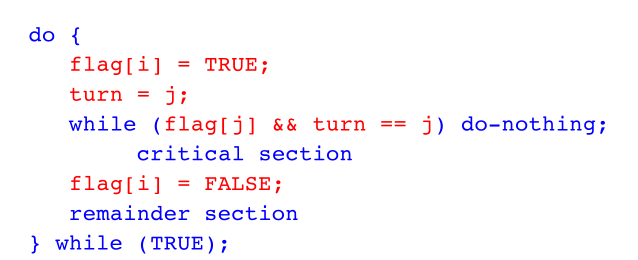
\includegraphics[scale = 0.7]{peterson.png}
	\bigbreak

	\begin{enumerate}
		\item Mutual exclusion is preserved.
		\item Progress requirement is satisfied.
		\item Bounded-waiting requirement is met.
	\end{enumerate}
\end{itemize}

\subsection{Synchronization Hardware}

\begin{itemize}
	\item Many systems provide hardware support for critical section code.
	\item \tf{Uniprocessors}
	\begin{itemize}
		\item Disable interrupts
		\item Currently running code would execute without preemption.
		\item Generally too efficient on multiprocessor systems.
	\end{itemize}

	\item Modern machines provide special atomic hardware instructions.
\end{itemize}

\subsection{Lock's Solution}

\begin{minted}{cpp}
	do{
		acquire lock
		critical section
		release lock

		remainder section
	} while(1);
\end{minted}

\begin{itemize}
	\item Peterson's Solution are not guaranteed to work on modern computer architecture.
	\item Any solution to the critical section problem requires a simple tool called \tf{lock}. 
\end{itemize}


\newpage
\section{Memory Management}

\subsection{Background}

\subsubsection{Basic Hardware}

\begin{itemize}
	\item Main memory and the registers that are built into each processing core are the only general-purpose storage that the CPU can access directly.
	\item Registers that are built into each CPU core are generally accessible within one circle of the CPU clock.
	\item Completing a memory access may take many cycles of the CPU clock. In such cases, the processor normally need to \tf{stall}, since it does not have the data required to complete the instruction that it is executing.
\end{itemize}

\bigbreak
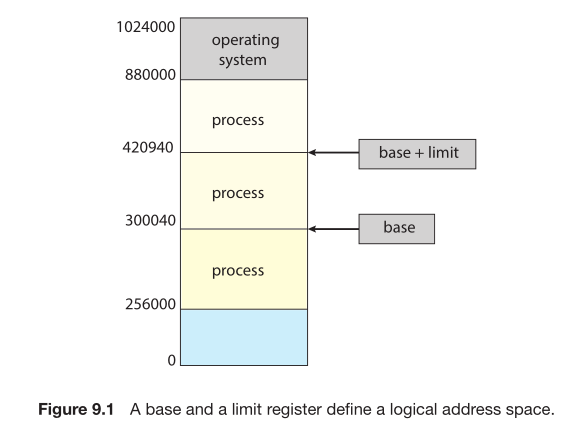
\includegraphics[scale = 0.7]{register.png}
\bigbreak

\par{For proper system operation, we must protect the operating system from access by user processes, as well as protect user processes from another}

\begin{itemize}
	\item Each process has a separate memory space, to separate memory spaces, we need the ability to determine the range of legal addresses that the process may access and to ensure that the process can access only these legal addresses => Using two register.
	\item The \tf{base register} holds the smallest legal physical memory address; the \tf{limit register} specifies the size of the range.
	\item  For example, if the base register holds 300040 and the limit register is 120900, then the program can legally access all addresses from 300040 through 420939 (inclusive).
	\item Protection of memory space is accomplished by having the CPU hardware compare every address generated in user mode with the registers.
	\item The base and limit registers can be loaded only by the operating system, which use the a special privileged instruction.
	\item The operating system is given \tf{unrestricted} access to both operating system memory and user memory.
\end{itemize}

\bigbreak
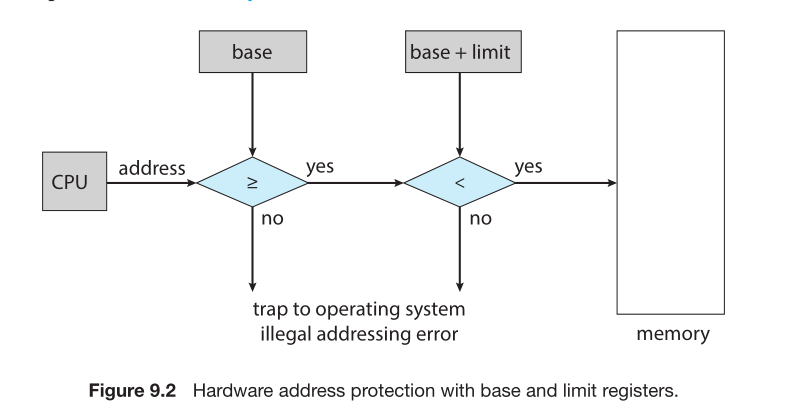
\includegraphics[scale = 0.7]{Harware-protection-register.png}
\bigbreak

\subsubsection{Address Binding}

\subsubsection{Logical and Physical Address Space}

\begin{itemize}
	\item An address generated by the CPU is commonly referred to as a \tf{logical address}
	\item An address seen by the memory unit - the one loaded into the \tf{memory-address register} of the memory - is called \tf{physical address}.
	\item Logical address is sometimes referred as \tf{virtual address}.
	\item All logical addresses is generated by a program called \tf{logical address space}, the set of all physical addresses corresponding to these logical addresses is a \tf{physical address space}.
	\item The run-time mapping from virtual to physical addresses is done by as hardware device called \tf{memory-management unit (MMU)}.
	
	\bigbreak
	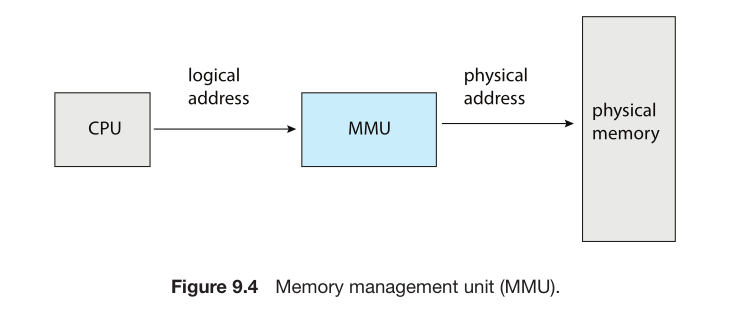
\includegraphics[scale = 0.7]{MMU.png}
	\bigbreak

	\item We now have two different types of addresses: logical addresses (in the range 0 to max) and physical addresses (in the range R + 0 to R + max for a base value R). The user program generates only logical addresses and thinks that the process runs in memory locations from 0 to max.
	\item  These logical addresses must be mapped to physical addresses before they are used.
	
	\bigbreak
	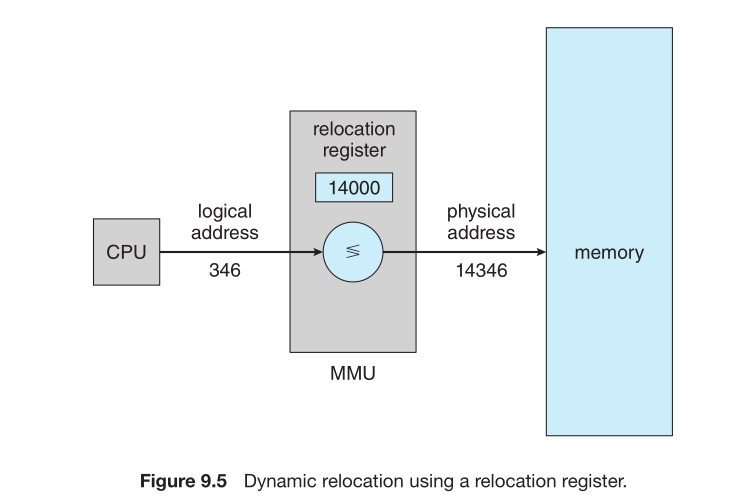
\includegraphics[scale = 0.7]{Dynamic-realocation.png}
	\bigbreak
\end{itemize}

\subsubsection{Dynamic Loading}

\par{The entire program and all data of a process to be in physical memory for the process to execute. The size of a process has thus been limited to the size of physical memory. To obtain better memory-space utilization, we can use \tf{dynamic loading}.}

\begin{itemize}
	\item A routine is not loaded until it is called. (advantage of dynamic loading)
	\item All routines are kept on disk in a relocatable load format.
	\item Dynamic loading does not require special support from operating system.
\end{itemize}

\subsubsection{Dynamic Linking and Shared Libraries}

\begin{itemize}
	\item \tf{Dynamically linked libraries (DLLs) are system libraries that are linked to user programs when the programs are run}
	\item \tf{Static Linking:} system libraries are treated like any other object module and are combined by the loader into the binary program image.
	\item \tf{Dynamic Linking:} linking is postponed until execution time.
\end{itemize}

\subsection{Contiguous Memory Allocation}

\par{The memory is usually divided into two partitions: one for operating system and one for the user processeses. The operating system can be either low memory addresses or high memory addresses. For Linux and Window the operating systems are placed in high memory.} \\

\par{In \tf{contiguous memory allocation}, each process is contained in a single section of memory that is contigous to the section containing the nest process.}

\subsubsection{Memory Protection}

\par{To prevent a process from accessing memory that it does not own, we use a relocation register and a limit register. The relocation register contains the smallest value of physical address; the limit register contains the range of the logical address.} \\

\par{Each logical addresss must fall within the range specified by the limit register.} \\

\bigbreak
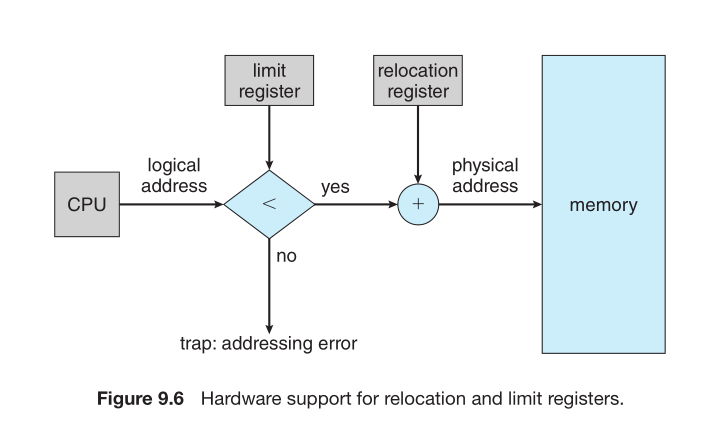
\includegraphics[scale = 0.7]{memory-protection.png}
\bigbreak

\subsubsection{Memory Allocation}

\par{One of the simplest methods of allocating memory is to assign processes to variably sized partitions in memory, where each partition may contain exactly one process.} \\

\bigbreak
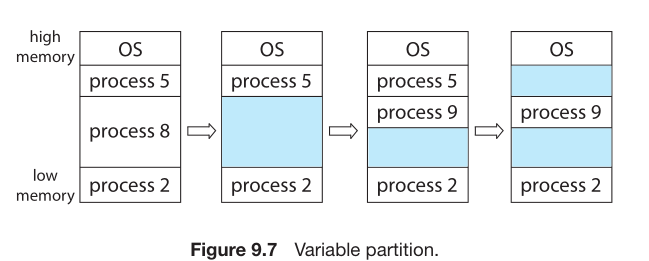
\includegraphics[scale = 0.7]{Variable_partition.png}
\bigbreak

\par{If there is not suffcient memory to satisfy the demands of an arriving process, such process will be placed in to a wait queue. When memory is later released, the operating system checks the wait queue to determine if it will satisfy the memory demands of a waiting process.} \\

\par{The memory comprise a \tf{set} of hole of various sizes scattered throughout memory. When a process arrives and needs memory, the system searches the set for a hole that is large enough for this process. If the hole is too large, it is split into two parts. One part is allocated to the arriving process; the other is returned to the set of holes. When a process terminates, it releases its block of memory, which is then placed back in the set of holes. If the new hole is adjacent to other holes, these adjacent holes are merged to form one larger hole.} \\

\par{The \tf{first-fit}, \tf{best-fit}, \tf{worst-fit} strategies are the ones most commonly used to select a free hole from the set of available holes.} \\

\begin{itemize}
	\item \tf{First-Fit:} Allocate the first hole that is big enough. Searching can start either at the beginning of the set of holes or at the location where the previous first-fit search ended. We can stop searching as soon as we find a free hole that is large enough.
	\item \tf{Best-Fit:} Allocate the smallest hole that is big enough. We must search the entire list, unless the list is ordered by size. This strategy produces the smallest leftover hole.
	\item \tf{Worst-Fit:} Allocate the largest hole. Again, we must search the entire list, unless it is sorted by size. This strategy produces the largest leftover hole, which may be more useful than the smaller leftover hole from a best-fit approach.
\end{itemize}

\par{Both first-fit and best-fit are better than worst-fit in terms of decreasing time and storage untilization. Neither first-fit nor best-fit is clearly better than the other in terms of storage ultilization, but first-fit is generally faster.}

\subsubsection{Fragmentation}

\begin{enumerate}
	\item \tf{External fragmentation:} exists when there is enough total memory space to satisfy a request but the available spaces are not contiguous: storage is fragmented into a large number of small holes. In the worst case, there is block of free(or wasted) memory between every two processes.
	\item Both the \tf{first-fit} and \tf{best-fit} strategies for memory allocation suffer from external fragmentation.
	\item \tf{Internal fragmentation:} unused memory that is \tf{internal} to a partition.
\end{enumerate}

\par{One solution for the external fragmentation is \tf{compaction}. The goal is to \tf{shuffle} the memory contents so as to place all free memory together in one large block. However it is only possible if relocation is dynamic and is done at the execution time.} \\

\par{Another possible solution is to permit the logical address space of processes to be noncontiguous, thus allowing a process to be allocated physical memory whereever such memory is available known as \tf{paging}.}

\subsection{Paging}

\par{\tf{paging}, a memory-management scheme that permits a process's physical address space to be non-contiguous. Paging avoids external fragmentation and the associated need for compaction.}

\subsubsection{Basic Method}

\par{The basic method for implement paging involves breaking physical memory into fixed-sized blocks called \tf{frames} and breaking logical memory into blocks of the same size called \tf{pages}.} \\

\par{When a process is to be executed,its pages are loaded into any available memory frames from their source (a file system or the backing store). The backing store is divided into fixed-sized blocks that are the same size as the memory frames or clusters of multiple frames.} \\ 

\par{Every address generated by the CPU is divided into two parts: a \tf{page number} (p) and a \tf{page offset} (d)} \\

\bigbreak
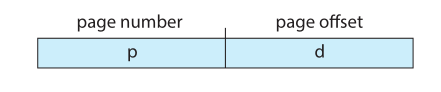
\includegraphics[scale = 0.7]{address-paging.png}
\bigbreak

\par{The page number is used as an index into a per-process \tf{pafe table}. The page table contains the base address of each frame in physical memory, and the offset is the location in the frame being referenced. The base address of the frame is combined with the page offset to define the physical memory address.} \\

\par{How the MMU translate a logical address generated by the CPU to a physical address:} \\

\begin{enumerate}
	\item Extract the page number \ti{p} and use it as an index into the page table.
	\item Extract the corresponding frame number \ti{f} from the page table.
	\item Replace the page number \ti{p} in the logical address with the frame number \ti{f}.
\end{enumerate}

\par{The page size (the frame size) is defined by the hardware. The size of the page is a power of 2, typically varying between 4 Kb and 1 GB per page, depending on the computer architecture.}

\par{If the size of the logical address space is $2^m$, and a page size is $2^n$ bytes, then the high order \ti{m - n} bits is a page number, and the n low-order bits is the page offset.} \\

\bigbreak
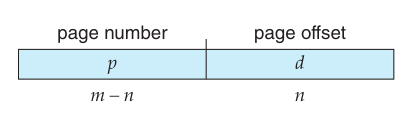
\includegraphics[scale = 0.7]{find-logic-address.png}
\bigbreak

\par{When we use a paging scheme, we have no external fragmentation: any free frame can be allocated to a process that needs it. However, we may face to some internal fragmentations.}

\par{If process size is indenpedent of page size, we expect internal fragmentation to average one-half page per process.}

\par{Pages is typically either 4 KB or 8 KB in size nowadays. On
x86-64 systems, Windows 10 supports page sizes of 4 KB and 2 MB . Linux also supports two page sizes: a default page size (typically 4 KB)and an architecture-dependent larger page size called \tf{huge pages}.}

\subsubsection{Hardware Support}

\par{page tables are per-process data structures, a pointer to the page table is stored with the other register values (like the instruction pointer) in the process conrol block of each process.} \\

\par{In the simplest case, the page table is implemented as a set of dedicated high-speed hardware registers, which makes the page-address translation very efficient. $\rarrow$ increase context-switch time, as each one of these registers must be exchanged during a context switch.} \\

\par{The page table is kept in \tf{main memory}, and a \tf{page-table base register (PTBR)} points to the page table.} \\

\par{Changing page table requires only change this register, substaintially reducing context-switch time.} \\

\begin{enumerate}
	\item \tf{Translation Loook-Aside Buffer (TLB)} \\
	
	\begin{itemize}
		\item A special, small, fast-lookup hardware cache.
		\item The TLB is associated and high-speed memory.
		\item Each entry in the TLB contains two parts: a key(or tag) and a value.
		\item The TLB must be kept small, typically between 32 and 1024 entries in size.
	\end{itemize}
\end{enumerate}

\par{The TLB is used with page tables in the following way. The TLB contains only a few of the page-table entries. When a logical address is generated by the CPU , the MMU first checks if its page number is present in the TLB . If the page number is found, its frame number is immediately available and is used to access memory.} \\

\par{IF the page table is not in the TLB (\tf{TLB miss)}, address translation will proceeds with a page table.} \\

\bigbreak
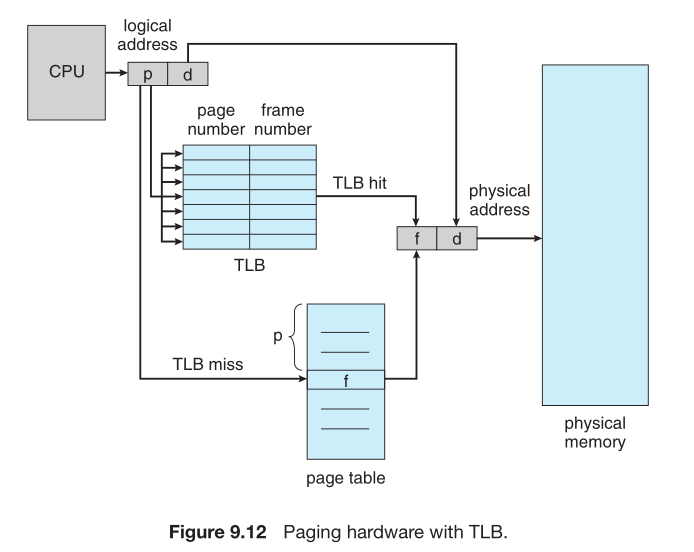
\includegraphics[scale = 0.7]{TLB.png}
\bigbreak

\par{if the TLB is already full of entries, an existing entry must be selected for replacement.} \\

\par{The percentage of times that the page number of interest is found in the TLB is called the \tf{hit ratio}}

\par{An 80-percent hit ratio, for example, means that
we find the desired page number in the TLB 80 percent of the time. If it takes 10 nanoseconds to access memory, then a mapped-memory access takes 10 nanoseconds when the page number is in the TLB . If we fail to find the page
number in the TLB then we must first access memory for the page table and frame number (10 nanoseconds) and then access the desired byte in memory (10 nanoseconds), for a total of 20 nanoseconds. The \tf{effective memory access time} (EAT) is:} \\

\begin{align}
	EAT &= 0.8 \times 10 + 0.2 \times 20 \\
		&= 12 nanoseconds 
\end{align}

\subsubsection{Protection}

\par{Memory protection implemented by associating protection bit with each frame to indicate if read-only or read-write is allowed.}

\par{At the same time that the physical address is being computed, the protection bis can be checked to verified that no writes are being made to a read-only page.}

\par{One additional bit is generally attached to each entry in the page table: a \tf{valid-invalid} bit.}

\begin{itemize}
	\item When this bit is set to \ti{valid}, the associated page is in the process's logical address space and is thus a legal (or valid) page.
	\item When the bit is set to \ti{invalid}, the page is not in the process's logical address space. Illegal addresses are trapped by use of the valid-invalid bit.
\end{itemize}

\par{Rerely does a process use all its address range. In fact, many processes use only a small fraction of the address space available to them.}

\par{Some system provide hardware, in the form of a \tf{page-table-length register (PTLR)}, to indicate the size of the page table. This value is checked against every logical address to verify that the address is in the valid range for the process}

\subsubsection{Shared Pages}

\begin{itemize}
	\item One copy of read-only (\tf{reentrant}) code shared among processes (Ex: text editors, compilers, window systems)
	\item Similar to multiple threads sharing the same process space.
	\item Useful for inter-process communication is sharing of read-only pages is allowed.
\end{itemize}

\subsection{Structure of the Page Table}

\subsubsection{Hierarchical Paging}

\begin{itemize}
	\item Most modern computer systems support a large logical address space ($2^{32} to 2^{64}$). $\rarrow$ the page table itself becomes excessively large.
	\item One way to solve this problem is use a two-level paging algorithm, in which the page table itself is also paged.
	\item For a system with a 64-bit logical address space, a two-level paging scheme is no longer appropriate.
\end{itemize}

\subsubsection{Hashed Page Tables}

\begin{itemize}
	\item One approach for handling address spaces larger than 32 bits is to use a \tf{hashed page table}, with the hash value being the virtual table number. 
	\item Each entry in the hash table contains a linked list of elements that hash to the same location (to handle collisions).
	\item Each element consists of three fields:
	\begin{itemize}
		\item The virtual page number.
		\item The value of the mapped page frame.
		\item A pointer to the next element in the linked list
	\end{itemize}

	\item The algorithm works as follows: The virtual page number in the virtual address is hashed into the hash table. The virtual page number is compared with field 1 in the first element in the linked list. If there is a match, the corresponding page frame (field 2) is used to form the desired physical address. If there is no match, subsequent entries in the linked list are searched for a matching virtual page number.
	
	\bigbreak
	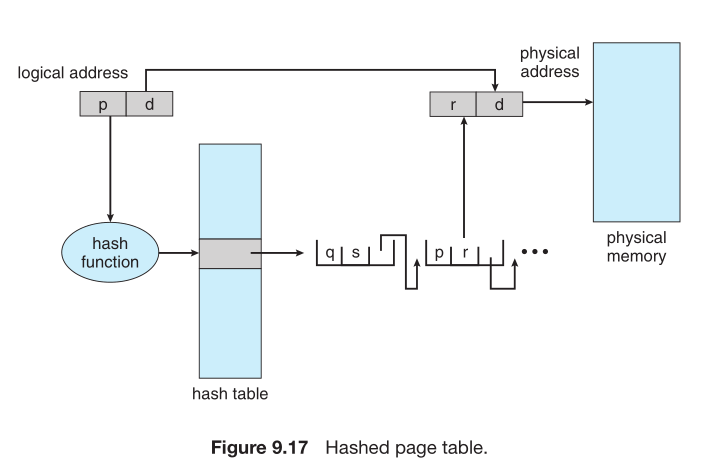
\includegraphics[scale = 0.7]{HashedPageTable.png}
	\bigbreak

	\item A variation of this scheme that is useful for 64-bit address spaces has been proposed. This variation uses clustered page tables, which are similar to hashed page tables except that each entry in the hash table refers to several pages (such as 16) rather than a single page.
\end{itemize}

\subsection{Swapping}

\begin{itemize}
	\item Process instructions and the data they operate on must be in memory to be executed. However, a process, or a portion of a process, can be \tf{swapped} temporarily out of memory to a \tf{backing store} and then brought back into memory for continue execution.
	
	\bigbreak
	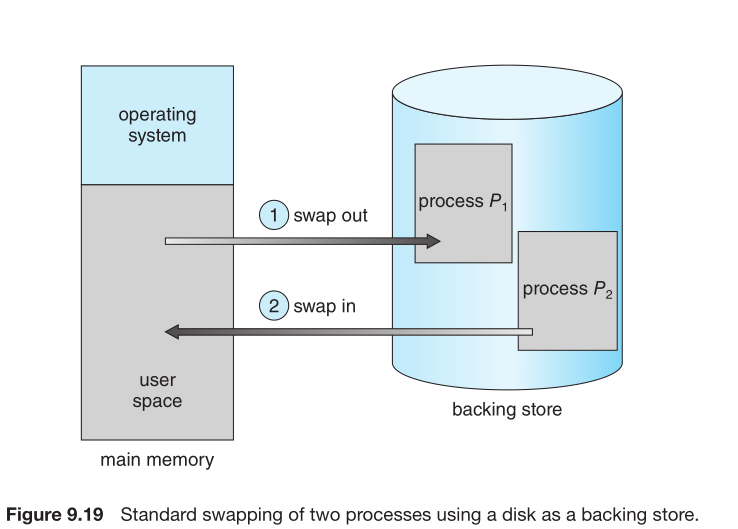
\includegraphics[scale = 0.7]{Swapping.png}
	\bigbreak

	\item Swapping makes it possible for the total physical address space of all processes to exceed the real physical memory of the system, thus increasing the degree of multiprogramming in a system.
	\item \tf{Roll in, roll out:} lower-priority process is swapped out so higher-priority process can be loaded and executed.
	\item System maintains a \tf{ready queue} of ready-to-run processes which have memory images on disk.
\end{itemize}

\subsection{Segmentation}

\begin{itemize}
	\item Memory-management scheme that supports user view of memory.
	\item A program is a collection of segments; A segment is a logical unit such as: main program, procedure, function, method, object, local variables, global variables, stack, etc.
\end{itemize}

\bigbreak
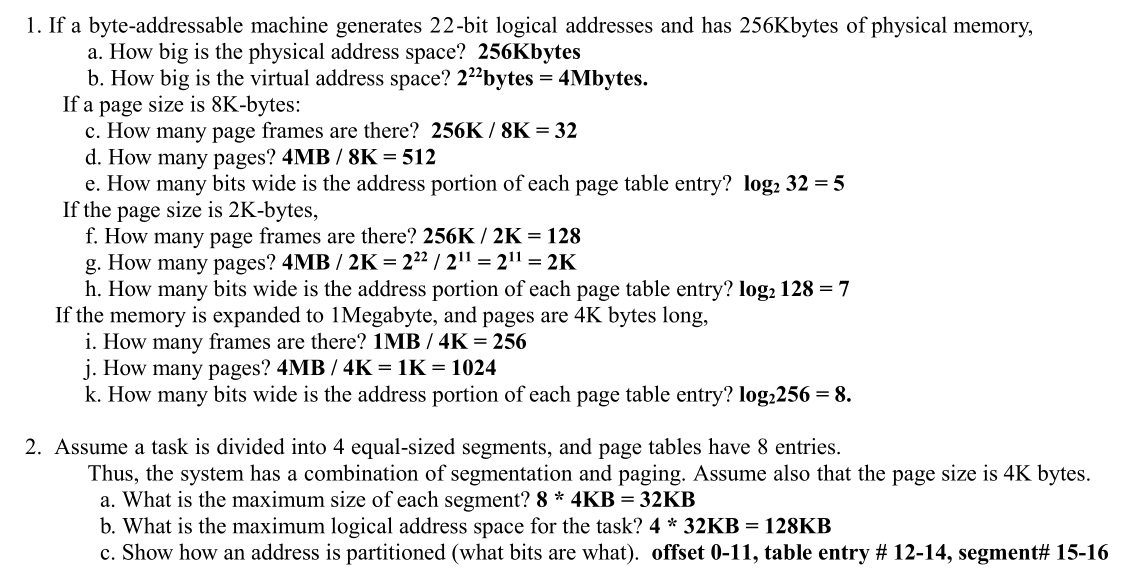
\includegraphics[scale = 0.7]{segment1.png}
\bigbreak

\bigbreak
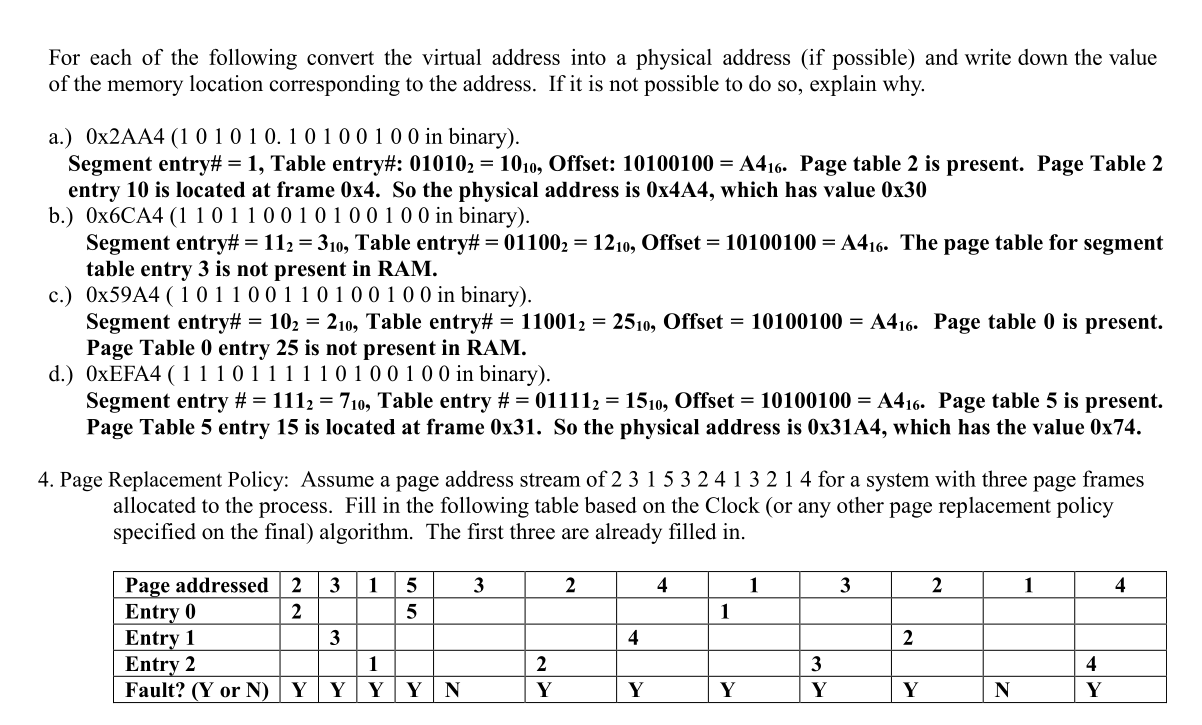
\includegraphics[scale = 0.7]{segment2.png}
\bigbreak

\newpage
\begin{center}
	Good Luck :) Myself
\end{center}

\end{document}